% !TeX TXS-program:compile = txs:///pdflatex/[--shell-escape]
\documentclass[tikz]{beamer}


\usepackage{minted}
\usepackage[parfill]{parskip}    		
\usepackage{graphicx}				
\usepackage{amssymb}
\usepackage{amsfonts}
\usepackage{amsmath}
\usepackage{bm}
\usepackage{tikz-cd}
\usepackage{enumerate}
\usepackage{xfrac}
\usepackage{hyperref}
\usepackage{graphicx} \graphicspath{ {./} }
\usepackage{xcolor}
\usepackage{bbold}


\newcommand{\cat}[1]{\bm{ \mathsf{#1} }}
\newcommand{\functor}[3]{#1 : \cat{#2} \to \cat{#3}}
\newcommand{\functordef}{\functor{F}{C}{D}}
\newcommand{\cc}{\cat{C}}
\newcommand{\dd}{\cat{D}}
\newcommand{\ee}{\cat{E}}
\newcommand{\subcat}[2]{\bm{ \mathsf{#1}}_{\bm{ \mathsf{#2}}}}
\newcommand{\op}[1]{#1^{\text{op}}}
\newcommand{\opc}{\op{\cc}}
\newcommand{\opd}{\op{\dd}}
\newcommand{\ope}{\op{\ee}}
\newcommand{\mono}{\rightarrowtail}
\newcommand{\epi}{\twoheadrightarrow}
\newcommand{\zero}{\bm{\mathbb{0}}}
\newcommand{\one}{\bm{\mathbb{1}}}
\newcommand{\two}{\bm{\mathbb{2}}}
\newcommand{\three}{\bm{\mathbb{3}}}
\newcommand{\bg}{\cat{BG}}
\newcommand{\bgg}{\cat{BG'}}
\newcommand{\nt}{\Rightarrow}
\newcommand{\ant}[2]{\alpha : F \nt G} 
\newcommand{\bnt}[2]{\beta : F \nt G} 
\newcommand{\anti}[2]{\alpha : F \cong G} 
\newcommand{\bnti}[2]{\beta : F \cong G} 
\newcommand{\red}[1]{\textcolor{red}{#1}}
\newcommand{\mred}[1]{\textcolor{red}{$#1$}}
\newcommand{\blue}[1]{\textcolor{blue}{#1}}
\newcommand{\mblue}[1]{\textcolor{blue}{$#1$}}


\setbeamertemplate{navigation symbols}{\insertframenumber{}}
\colorlet{shadecolor}{gray!15}
\usepackage[utf8]{inputenc}
\usepackage[english]{babel}
\newcommand{\propnumber}{} % initialize
\newtheorem*{prop}{Proposition \propnumber}
\theoremstyle{definition}
\newtheorem{defn}{Definition}[section]

\AtBeginSection[]{
  \begin{frame}
  \vfill
  \centering
  \begin{beamercolorbox}[sep=8pt,center,shadow=true,rounded=true]{title}
    \usebeamerfont{title}\insertsectionhead\par%
  \end{beamercolorbox}
  \vfill
  \end{frame}
}

\begin{document}
\title{Hulk Smash}
\author{Emily Pillmore}

\frame{\titlepage}

\section[Outline]{}
\frame{ \tableofcontents[hideallsubsections] }

\section{Introduction}
\subsection{Who am I?}

\frame
{
	My name is Emily Pillmore.
	
	I am a Haskell and Math enthusiast. Trying to be more of the latter, less of the former lately.
}

\frame
{
	\begin{itemize}
		\item Twitter (\href{https://twitter.com/pitopos}{@pitopos})
		\item Meetups in NYC: NY Homotopy Type Theory, NY Category Theory, and the NY Haskell User Group. 
		\item Meetups in Asheville: Asheville Functional Programming Groups, Asheville Category Theory (only member :'()
		\item Discord: Haskell $\cap$ Dank Memes: \href{https://discord.gg/2x2fYSK}{https://discord.gg/2x2fYSK}. 
		\item Personal: All of my slides and meetup content are hosted at \href{https://github.com/cohomolo-gy}{cohomolo.gy}.
	\end{itemize}
	
	
	If you ever want to talk category theory or programming, I'm around to talk, help, etc. 
}

\frame
{
	I got my start in Scala, with Runar's \textit{Functional Programming in Scala} (the \textcolor{red}{red one} - there is now a \textcolor{blue}{blue one})
	\\
	\\
	I work in Haskell pretty exclusively now, recreationally with Coq and Lean.
}


\frame
{ 
	I work at a company called \textbf{Kadena}, designing a language, a private permissioned blockchain, and a public one.
	\begin{center}
		
\includegraphics[scale=0.4]{kadena}
	\end{center}
	
}

\subsection{Why are we here?}
\frame
{
	\begin{itemize}
		\item A lite talk to end the day - nothing too serious or strenuous
		\item To learn a bit more about the Maybe monad than you probably knew prior to this talk
		\item See an interesting geometric perspective on the subject
		\item Take away some inspiration for thinking about types in Haskell
		\item Have fun and spread the... like.
		
	\end{itemize}
}

\subsection{And most importantly...}
\frame
{
To enjoy ourselves 

	\begin{center}
		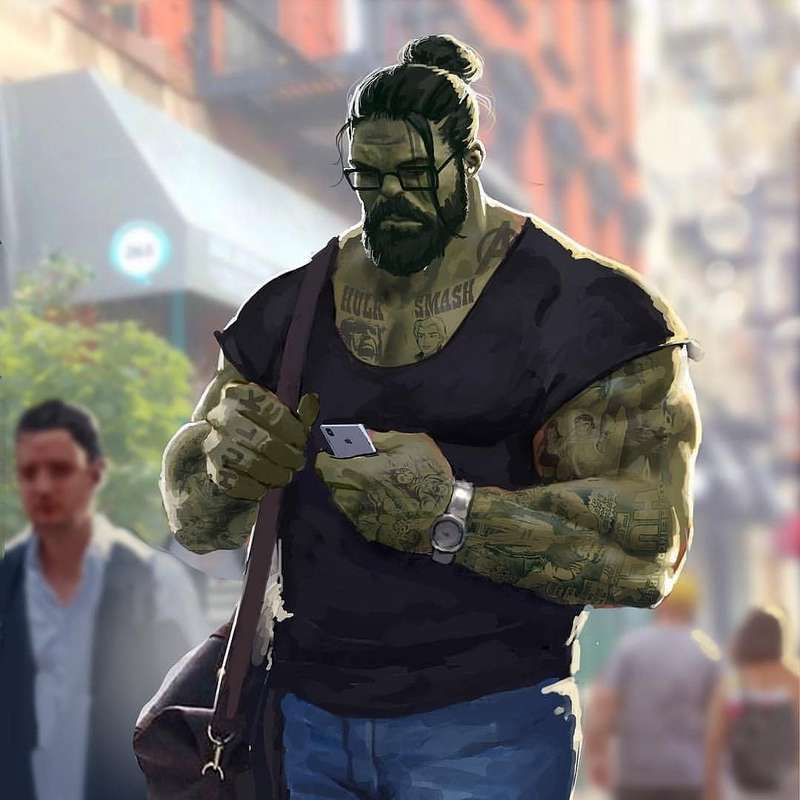
\includegraphics[scale=0.25]{tender_hulk}
	\end{center}
}

\section{Some Geometry}
\subsection{Pointed spaces}

\frame
{
In classical point-set topology we often consider topology and geometry in terms of sets of points.  
}

\frame
{
Often, we consider geometric objects with a particular "distinguished" base point picked out for us. 

\begin{center}
\begin{tikzpicture}
  \draw[color=red!60] (0,0) circle (2cm);
  \filldraw[black] (2,0) circle (2pt) node[anchor=west] {\mred{a_0}};
\end{tikzpicture}
\end{center}
}

\frame
{
Often, we consider geometric objects with a particular "distinguished" base point picked out for us. 

\begin{center}
\begin{tikzpicture}
  \draw[color=red!60] (0,0) circle (2cm);
  \filldraw[black] (2,0) circle (2pt) node[anchor=west] {\mred{a_0}};
\end{tikzpicture}
\end{center}

we can think of this as a pair of a geometric object and a base point \mred{(A, a_0)}.
}

\subsection{Products and Coproducts}

\frame
{
	We can build our usual product, coproduct and quotient spaces, and we can use the action of the base point to orient ourselves within the space.
}

\frame
{
	Products are relatively simple. We want to build a cartesian product of spaces as you already know how to do. 
	
	\begin{center}
		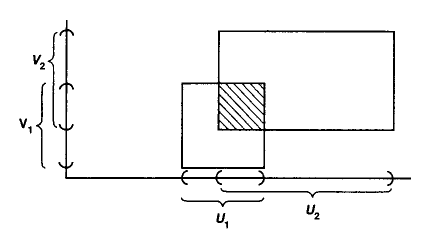
\includegraphics[scale=0.3]{product}
	\end{center}
	
	\begin{center}
		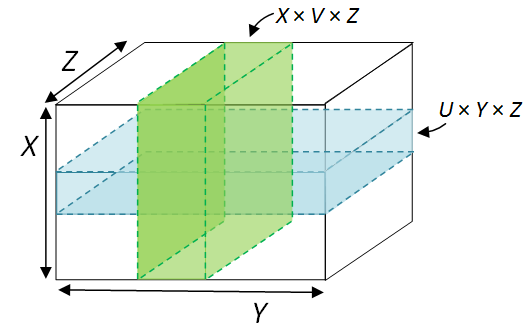
\includegraphics[scale=0.3]{product3}
	\end{center}
}

\frame
{
	What would a point look like in this product space? A pointed product? coproduct? A pointed coproduct?
}

\subsection{Quotient spaces}
\frame 
{
        	Quotient spaces are spaces built by identifying points according to some relation. Get ready for some bad paper-taping action
}

\frame 
{
	Some quotients can be very simple. For instance, the wedge sum (pointed coproduct) of two spaces is built by identifying the distinct basepoints of each object. We use the notation $X \vee Y$. When the objects are 1-spheres, we call this a \textit{topological rose}.
	
	\begin{center}
		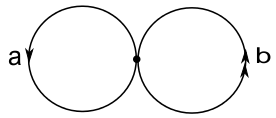
\includegraphics[scale=0.5]{wedge}
	\end{center}
	
	\begin{center}
		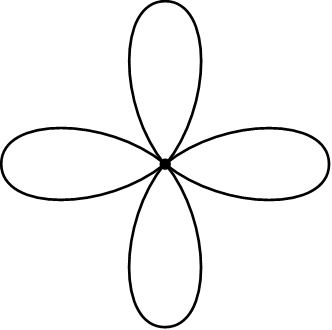
\includegraphics[scale=0.3]{rose}
	\end{center}
	
}

\frame
{
	Other quotients can be more complex. For example, consider the square torus $\mathbb{T}  \cong [0,1] \times [0,1] / (x,0) \sim (x,1), (0, y) \sim (1, y)$: 
	
	\begin{center}
		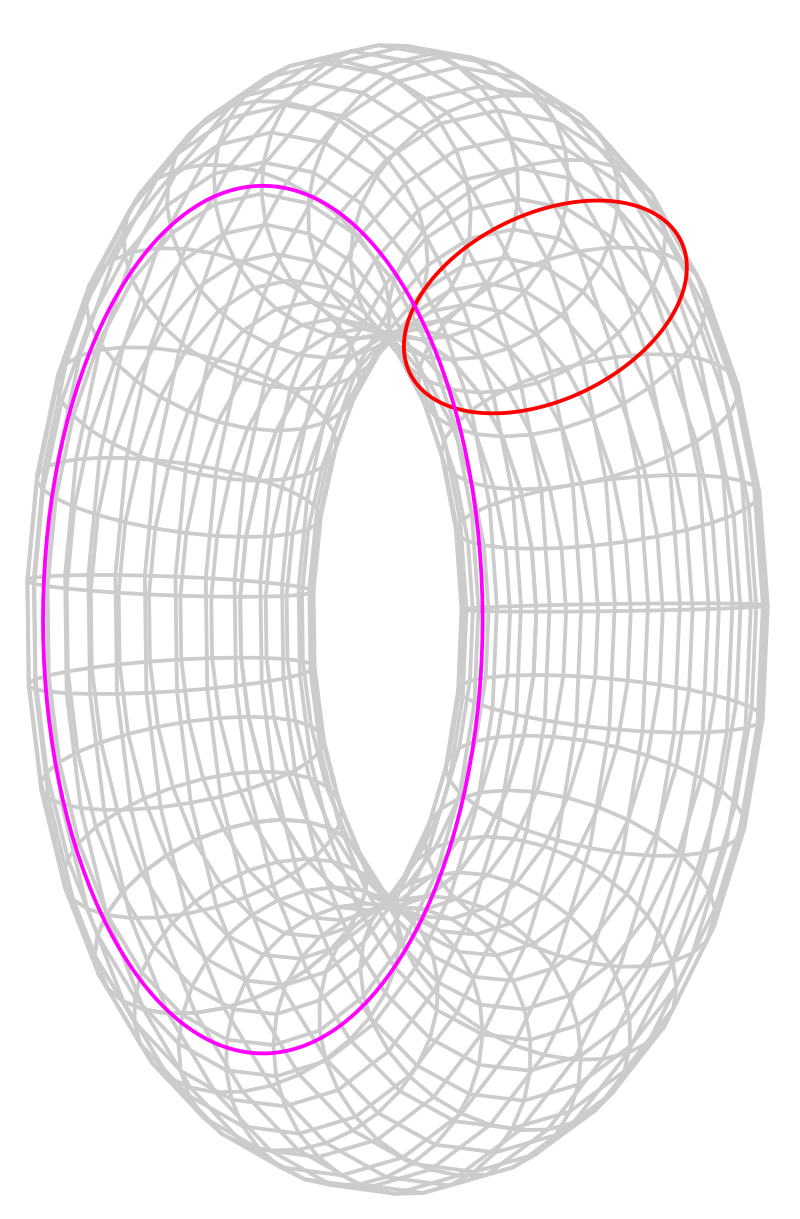
\includegraphics[scale=0.1]{torus_skeleton}
	\end{center}
	 
}

\frame
{
	If you want to try it yourself, it's actually quite easy with some paper and tape: 
	
	\begin{center}
		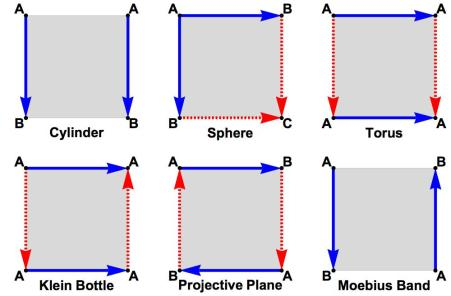
\includegraphics[scale=0.4]{identification_spaces}
	\end{center}
	 
}

\subsection{Smash products}
\frame
{
	I'd be remiss not to mention the \textit{smash product}, or \textit{collapsed product} - the quotient space of a product by a wedge sum. Formally, the smash product $X$ and $Y$ is the quotient $X \wedge Y := X \times Y / X \vee Y$
}

\section{Translation to Haskell}

\frame 
{
	In Haskell, we have discrete analogues of these constructions available to us, but first, we must consider the monad in which we will work: the \textbf{Maybe} monad. 

}

\begin{frame}[fragile]
	
	\begin{center}
		\begin{minted}[]{haskell}
data Maybe a = Just a | Nothing
			
instance Functor Maybe where
  fmap f Nothing = Nothing
  fmap f (Just a) = Just (f a)
			  
instance Applicative Maybe where
  pure = Just
		  
  Just f <*> a = fmap f a
  Nothing <*> _ = Nothing
			  
instance Monad Maybe where
  return = Pure
  
  Just a >>= f = f a
  Nothing >>= _ = Nothing
\end{minted}
\end{center}
\end{frame}

\frame
{
	The \textbf{Maybe} monad corresponds with the map $A \mapsto  A \sqcup *$, which can be thought of as "adjoining a basepoint" to $A$. We can consider $\mathbf{Maybe A}$ to be a "pointed object" in the precise that it is an object of \textbf{Hask} equipped with a disjoint basepoint. 
}

\frame
{
 	Using this fact, we can draw a direct line from point-set topology and the objects we just discussed to Haskell types, using a general notion of "pointed", and looking to category theory and type arithmetic. 
}


\begin{frame}[fragile]
	Products of pointed spaces have a straightforward calculus (technically, abusing RAPL/LAPC/Yoneda all over the place):  
	
	\begin{minted}[]{haskell}
	(Maybe a, Maybe b)
	-- simplifying notation
	~ (1 + a) * (1 + b)
	-- products distribute over coproducts
	~ 1 + b + a + a*b
	-- associativity
	~ 1 + (a + b + a*b)
	~ Maybe (Either a (Either b (a,b)))
	\end{minted}
\end{frame}

\frame
{
	Those in the know will recognize the term $a + b + a*b$ as the \textbf{These} datatype.
}

\begin{frame}[fragile]
\begin{center}
	\begin{minted}[]{haskell}
	data These a b 
	  = This a
	  | That b
	  | These a b
	\end{minted}
\end{center}
\end{frame}

\frame
{
	More on \textbf{These} later. But, to recap, a "product of pointed objects" is isomorphic to \textbf{Maybe (These a b)}.
}

\frame
{
	Pointed coproducts are slightly easier. A pointed coproduct is a coproduct of pointed objects, but with the base point identified. Intuition: attaching a basepoint to the usual coproduct diagrams.
}

\begin{frame}[fragile]
\begin{center}
	\begin{minted}[]{haskell}
	Either (Maybe a) (Maybe b)
	-- simplification of notation
	~ (1 + a) + (1 + b)
	-- basepoints are identified 
	-- via the pushout: a0 <- * -> b0
	~ 1 + a + b
	-- assocativity
	~ 1 + (a + b)
	~ Maybe (Either a b)
	\end{minted}
\end{center}
\end{frame}

\frame
{
	This is precisely the shape of a wedge sum, like the topological rose we just saw!
}

\frame
{
	We can even form an analogue of the smash product we build. Recall that the \textit{smash product} of $X$ and $Y$ is the quotient of the product by a wedge: $X \wedge Y := X \times Y / X \vee Y$.
}

\begin{frame}[fragile]
\begin{minted}{haskell}
(Maybe a, Maybe b) / Maybe (Either a b)
-- notation
~ (1 + a) * (1 + b) / (1 + a + b)
-- defn + reassociate
~ (1 + a + b) + a*b / (1 + a + b)
-- quotient (1 + a + b) ~ * - note that
-- this means 'identify to a point', not divide!
~ 1 + a*b
~ Maybe (a,b)
\end{minted}
\end{frame}

\frame
{
	This means to build the geometry above, we need the following three datatypes (forgive the names)
}
\begin{frame}[fragile]
\begin{minted}{haskell}
data Can a b = Non | One a | Eno b | Two a b
data Wedge a b = Nada | Here a | There b
data Smash a b = Nothing | Smash a b
\end{minted}
\end{frame}

\frame
{
	So this is pretty interesting! We're not actually skimping on details to build this calculus, just some good knowledge of how pointed objects work, and geometry to guide our intuition.
}

\frame
{
	CT Aside: When the ambient category is closed monoidal, smash products form a separate monoidal tensor in its category of pointed objects, with its own base point-preserving analogue to currying, uncurrying (see: basepoint-preserving function spaces), and the usual distributivity over pointed coproducts (Wedges) and symmetry + associativity that one might expect. When the ambient category is additionally symmetric , the smash product is also symmetric.
	  
}


\section{What about These?}

\frame
{
	What's up with \textbf{These}? It doesn't really seem to fit in: 
	
	\begin{itemize}
		\item It's got no "basepoint" to speak of
		\item There's no real good intuition for it, unlike the rest other than maybe "inclusive union"
		\item It was originally developed to encapsulate "zippy" behavior.
		\item How can we think of it beyond being a "convenient data type that fits with our ad hoc needs"?
		\item Is \textbf{These} to the pointed product as \textbf{Semigroup} is to \textbf{Monoid}?
	\end{itemize}
}

\frame
{
	Fact: \textbf{These} is not so ad hoc as it might seem. In fact, there's some principles hiding behind the scenes.
}

\frame
{
	The encoding we've been implicitly using to denote "pointed objects" has been: 
	
	\begin{itemize}
		\item objects are pairs $(A, a_0)$
		\item morphisms $f : A \rightarrow B$ such that $f a_0 = b_0$. 
	\end{itemize}
	

However, there is an alternate encoding that is equivalent.
		
}

\frame
{
	Consider this equivalent encoding of pointed spaces: 
	\begin{itemize}
		\item objects are the same
		\item morphisms $f : A \rightarrow B \sqcup *$
	\end{itemize}
	
}

\frame
{
	These encodings are, in a loose sense, equivalent by the following functor $\mathbf{F}$: 
	
	\begin{itemize}
		\item For objects: $FA = (A \sqcup *, *)$
		\item For morphisms $f : A \rightarrow B \sqcup * = (>>= f) $
		\item and any morphism $g : A \sqcup * \rightarrow B \sqcup *$ which satisfies $g* = *$ corresponds with $f$ such that $g = (>>= f)$ 
	\end{itemize}
}	

\frame
{
	Note: this is "loose" in the sense that types are not sets and one must treat them like they are to make that equivalence work. In the first encoding, $(Int \rightarrow Int, id)$ is an object, but there's no type $A$ such that $A \sqcup * ~ Int \rightarrow Int$.
}

\frame
{
	So what is \textbf{These}? Another way of encoding the pointed product, using the Kleisli category of the `Maybe` monad. 
}

\frame
{
	Which is nicer? You decide.
}

\section{Tying it all together}

\subsection{postlogue}
\frame
{
	Geometry gives us great intuition to draw from.
}

\frame
{
	We can look to Category theory not just to generalize and abstract our results, but translate across mathematical fields and boundaries. 
}

\frame
{
	Take ideas from everywhere, filter through category theory and sort into whatever hat you want to wear.
}

\frame
{
	All of these constructs are encapsulated in the \href{https://github.com/emilypi/smash}{smash} suite of libraries. 
}

\frame
{
	Feel free to contribute. There's lots of work to be done in terms of implementing monad transformers, optics, fun combinators etc. 
}

\subsection{fin}
\frame
{
	Thanks to Mniip for making the offhand comment that started me on this kick. And thanks to Haskell Love for tolerating me!
	\newline
	\begin{center}
		
\includegraphics[scale=0.35]{haskell_love}
	\end{center}
	 
}


\end{document}
